\documentclass[aspectratio=169,11pt]{beamer}

% Shared style (ib-tutorials.sty at the repo root).
\makeatletter\def\input@path{{./}{../}}\makeatother
\usepackage{ib-tutorials}

\usepackage[utf8]{inputenc}
\usepackage{amsmath,amssymb}
\usepackage{booktabs}
\usepackage{array}
\newcolumntype{L}[1]{>{\raggedright\arraybackslash}p{#1}}
\usepackage{graphicx}
\graphicspath{{../pictures/3-ibamr-fundamentals/}{pictures/3-ibamr-fundamentals/}}
\usepackage{xcolor}
\usepackage{listings}
\usepackage{tikz}
\usetikzlibrary{arrows.meta,positioning,shapes.geometric,fit,calc}
\usepackage{hyperref}

\newcommand{\sourcecredit}[1]{\vfill\begin{flushright}\tiny\textcolor{DarkGray}{#1}\end{flushright}}

\lstset{
  basicstyle=\ttfamily\scriptsize\color{BlackGray},
  keywordstyle=\color{NavyBlue}\bfseries,
  commentstyle=\color{DarkGray}\itshape,
  stringstyle=\color{OliveGreen},
  showstringspaces=false,
  columns=fullflexible,
  keepspaces=true,
  breaklines=true,
  breakindent=1em,
  frame=single,
  framerule=0.4pt,
  rulecolor=\color{LightGray},
  backgroundcolor=\color{LightGray!30},
  xleftmargin=0.25em,
  xrightmargin=0.25em
}
\lstdefinestyle{shell}{morecomment=[l]{\#}}
\lstdefinestyle{input}{morecomment=[l]{//}}
\lstdefinestyle{matlab}{morecomment=[l]{\%}}
\lstdefinestyle{python}{morecomment=[l]{\#}}
\lstdefinestyle{data}{}
\lstdefinestyle{tiny}{basicstyle=\ttfamily\tiny\color{BlackGray}}
\lstdefinestyle{inputtiny}{morecomment=[l]{//},basicstyle=\ttfamily\tiny\color{BlackGray}}
\lstdefinestyle{matlabtiny}{morecomment=[l]{\%},basicstyle=\ttfamily\tiny\color{BlackGray}}
\lstdefinestyle{pythontiny}{morecomment=[l]{\#},basicstyle=\ttfamily\tiny\color{BlackGray}}
\lstdefinestyle{cpp}{language=C++,morecomment=[l]{//}}
\lstdefinestyle{cpptiny}{language=C++,morecomment=[l]{//},basicstyle=\ttfamily\tiny\color{BlackGray}}
\lstdefinestyle{cmake}{morecomment=[l]{\#}}

\title[3D simulations]{3D simulations}
\subtitle{What changes in three dimensions: the input file's six sides, structures as sheets and bristles, the cost, and the 3D examples of this series}
\author[Miller]{Laura A. Miller}
\institute[UArizona]{Department of Mathematics, University of Arizona}
\date{Using IB Software \textbullet\ Part III \textbullet\ Chapter 12}

\begin{document}

% 1
\begin{frame}[plain]
\maketutorialtitlepanel{%
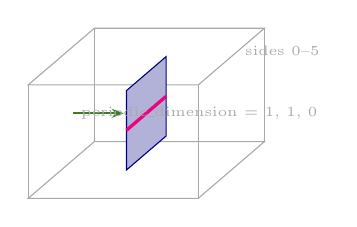
\begin{tikzpicture}[scale=0.8,x={(0.9cm,0)},y={(0.35cm,0.3cm)},z={(0,0.9cm)}]
  \draw[DarkGray] (0,0,0) -- (3,0,0) -- (3,3,0) -- (0,3,0) -- cycle;
  \draw[DarkGray] (0,0,2) -- (3,0,2) -- (3,3,2) -- (0,3,2) -- cycle;
  \draw[DarkGray] (0,0,0) -- (0,0,2); \draw[DarkGray] (3,0,0) -- (3,0,2); \draw[DarkGray] (3,3,0) -- (3,3,2); \draw[DarkGray] (0,3,0) -- (0,3,2);
  \fill[NavyBlue!30,draw=NavyBlue] (1.5,0.6,0.3) -- (1.5,2.4,0.3) -- (1.5,2.4,1.7) -- (1.5,0.6,1.7) -- cycle;
  \draw[RubineRed,very thick] (1.5,0.6,1.0) -- (1.5,2.4,1.0);
  \draw[-{Stealth[length=1.5mm]},OliveGreen,thick] (0.2,1.5,1.0) -- (1.1,1.5,1.0);
  \node[font=\tiny,text=DarkGray] at (1.5,3.9,0.2) {\code{periodic\_dimension = 1, 1, 0}};
  \node[font=\tiny,text=DarkGray] at (3.9,1.5,2.1) {sides 0--5};
\end{tikzpicture}}
\end{frame}

% 2
\begin{frame}{Learning goals}
\label{fr:goals}
\footnotesize By the end of this chapter you should be able to:
\begin{enumerate}
  \item write a 3D input file: three numbers wherever 2D had two, six sides numbered 0 to 5 in the boundary-condition blocks, a third velocity component with its own block, and a domain that need not be a cube;
  \item build a 3D structure file set (points with $x\,y\,z$, springs and beams along two directions of a sheet, target points along a line) and move its target points in 3D, as the course's leaf and moving plates did;
  \item run the 3D examples of this series, IB/08 (a bristle in a sheared box, target points) and IBFE/10 (a plate in a flow tank, finite elements), and say what each shows;
  \item estimate what a 3D run costs in cells, steps and cores, and why adaptive refinement and a short first run are not optional;
  \item find the 3D output (three numbers per point in \code{hier\_data\_IB3d}; \code{viz\_IB3d} for VisIt) and know where chapter 27 takes it.
\end{enumerate}
\begin{punchbox}
\footnotesize Nothing in the IB method changes between 2D and 3D; the delta function has a third factor and every array a third component. What changes is the cost, and the number of places where a third number has to be right.
\end{punchbox}
\end{frame}

% 3
\begin{frame}{How this chapter was checked}
\label{fr:checked}
\begin{itemize}\footnotesize
  \item The two 3D examples (IB/08 glycocalyx, IBFE/10 flow-tank plate) build and run with IBAMR 0.16.0 and 0.19.0; their READMEs record the numbers quoted here. The side numbering and the input keys are those of the current \code{muParserRobinBcCoefs} and \code{CartesianGeometry} input blocks, as read by those runs.
  \item The 2016 lecture \emph{3D Simulations} (public folder 8) is quoted in full; its 3D leaf example was a Google Drive link that no longer resolves, so the sheet is described from the slides and IB/08 stands in for the hands-on part.
  \item The 2012 lab ReadMe deck (the \code{moving\_plates2d}/\code{moving\_plates3d} clap-and-fling model, kinematics in \code{update\_target\_point\_positions.C}, the wing's four files and the generator run twice) is quoted; the 3D wing files and the lab's 2014 wing-mesh scripts (Ellington's planform) exist in the lab folders and are described, not shipped.
  \item The 2013 \emph{Math769 3D} deck in the course folders is in a format that no current tool can open; nothing from it is claimed here.
  \item A student's 2012 ``how to use 3D IBAMR'' deck is a walk-through of ssh, emacs and \code{screen} on a lab machine; its one technical line (\code{mpirun -np 4 ./main3d input3d}) is in chapter 1's terms already.
\end{itemize}
\begin{punchbox}
\footnotesize Slide numbers refer to this deck; chapter numbers (1, 5, 6, 7, 9a, 11, 16, 18, 22, 27, 28) to the other chapters of this series.
\end{punchbox}
\end{frame}

% 4
\begin{frame}{Where to look things up}
\label{fr:lookup}
\small
\begin{itemize}
  \item \al{The examples}: \code{examples/IB/08-glycocalyx-3d} (\code{input3d}, \code{generate\_mesh3d.py}/\code{.m}, \code{update\_target\_point\_positions.cpp}, README with the shear-flow timing) and \code{examples/IBFE/10-flow-tank-plate-3d} (\code{input3d}, \code{plate2.msh}, README); chapter 22 for the latter's physics.
  \item \al{Upstream 3D examples}: \code{examples/IB/explicit/ex7} (3D posts held by target points, IB/08's relative); \code{examples/IBFE/explicit/ex4} and \code{ex5} in 3D (IBFE/10's relatives); chapter 15's tour.
  \item \al{The input blocks}: chapter 7 (boundary conditions) for the Robin form and the \code{VelocityBcCoefs\_d} blocks; this chapter for the six sides and the third component.
  \item \al{Structure files in 3D}: chapter 6 (the formats are the same with three coordinates); IB/08's generator for a cylinder of rings; chapter 18 for finite-element meshes (gmsh).
  \item \al{Visualization}: chapter 27 (VisIt in 3D: slices, isosurfaces, the 2D slice from a 3D run) and chapter 28 (finite-element data).
  \item The IBAMR documentation, \url{https://ibamr.github.io/docs}; the FAQ, \url{https://github.com/IBAMR/IBAMR/wiki/FAQ}.
\end{itemize}
\end{frame}

% 5
\begin{frame}{The course's goal: a 3D leaf}
\label{fr:leaf}
\begin{columns}[T,onlytextwidth]
\begin{column}{0.58\textwidth}
\small From the 2016 lecture \emph{IBAMR boundary conditions / 3D simulations} (public folder 8): ``Our goal will be to develop a 3D simulation of a flexible `leaf'. The leaf will be tethered to target points along its midline and immersed in flow.''
\vspace{1mm}

\small ``\al{Rectangular sheet in flow.} In this case the leaf is simply a rectangle constructed from beams and springs. Target points along the centerline hold it in place. The matlab file \code{generate\_mesh3d.m} makes the necessary files.''
\vspace{1mm}

\footnotesize The 2016 slides showed the sheet twice: a rendering of the bent sheet in the stream, and the generator's picture of the flat rectangle of points with the centreline marked. The example's files were on a Google Drive link that no longer resolves; the sheet is rebuilt in words on slide \ref{fr:sheet}, and IB/08 (slide \ref{fr:ib08}) is the 3D example you can run.
\end{column}
\begin{column}{0.4\textwidth}
\centering
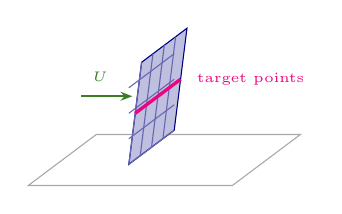
\begin{tikzpicture}[scale=0.9,x={(0.9cm,0)},y={(0.4cm,0.3cm)},z={(0,0.9cm)}]
  \draw[DarkGray,thin] (0,0,0) -- (3.2,0,0) -- (3.2,2.4,0) -- (0,2.4,0) -- cycle;
  \fill[NavyBlue!25,draw=NavyBlue] (1.4,0.4,0.2) -- (1.4,2.0,0.2) -- (1.6,2.0,1.8) -- (1.6,0.4,1.8) -- cycle;
  \foreach \y in {0.4,0.8,...,2.0}{\draw[NavyBlue!60,thin] (1.4,\y,0.2) -- (1.6,\y,1.8);}
  \foreach \z in {0.2,0.6,...,1.8}{\draw[NavyBlue!60,thin] (1.4,0.4,\z) -- (1.4,2.0,\z);}
  \draw[RubineRed,very thick] (1.5,0.4,1.0) -- (1.5,2.0,1.0);
  \draw[-{Stealth[length=1.5mm]},OliveGreen,thick] (0.3,1.2,1.0) -- (1.1,1.2,1.0);
  \node[font=\tiny,text=OliveGreen] at (0.6,1.2,1.3) {$U$};
  \node[font=\tiny,text=RubineRed] at (2.6,2.0,1.0) {target points};
\end{tikzpicture}

\scriptsize The 2016 sheet, redrawn: a rectangle of points joined by springs and beams along both directions, held by a line of target points along its middle, in a stream.
\end{column}
\end{columns}
\end{frame}

% 6
\begin{frame}{Review: Robin boundary conditions}
\label{fr:robin}
\small ``Robin boundary conditions are a weighted combination of Dirichlet boundary conditions and Neumann boundary conditions. If $\Omega$ is the domain on which the given equation is to be solved and $\partial\Omega$ denotes its boundary, the Robin boundary condition is
\[
  a\,u + b\,\frac{\partial u}{\partial n} = g \quad\text{on } \partial\Omega
\]
for some non-zero constants $a$ and $b$ and a given function $g$ defined on $\partial\Omega$.'' (2016)
\vspace{2mm}

\footnotesize Chapter 7 has the whole story: IBAMR's \code{acoef}, \code{bcoef} and \code{gcoef} functions are these $a$, $b$ and $g$, one set per velocity component and per side, and IBAMR's solver reads only the two pairs $(a, b) = (1, 0)$ (a value) and $(0, 1)$ (a normal derivative); anything in between is not a boundary condition it can apply. In 3D nothing changes but the count: three components, six sides.
\end{frame}

% 7
\begin{frame}[fragile]{IBAMR's boundary numbering in 3D}
\label{fr:sides}
\begin{columns}[T,onlytextwidth]
\begin{column}{0.5\textwidth}
\small ``Look in the \code{input3d} file.
\begin{itemize}
  \item 2D: \code{xleft = 0}, \code{xright = 1}, \code{ybottom = 2}, \code{ytop = 3}
  \item 3D: add \code{zbottom = 4}, \code{ztop = 5}.'' (2016)
\end{itemize}
\vspace{1mm}
\footnotesize The rule behind the numbers: side $2d$ is the lower end of direction $d$ and side $2d + 1$ the upper end ($d = 0, 1, 2$ for $x, y, z$). The 2016 slide drew the box with the six numbers on its faces; the sketch here is the same.
\begin{lstlisting}[style=inputtiny]
// one block per velocity component, six functions of each kind
VelocityBcCoefs_2 {                 // the z-component (IB/08)
   acoef_function_0 = "1.0"         // side 0: x lower
   acoef_function_1 = "1.0"         // side 1: x upper
   acoef_function_2 = "1.0"         // side 2: y lower
   acoef_function_3 = "1.0"         // side 3: y upper
   acoef_function_4 = "1.0"         // side 4: z lower (the floor)
   acoef_function_5 = "1.0"         // side 5: z upper (the lid)
   bcoef_function_0 = "0.0"  ...    bcoef_function_5 = "0.0"
   gcoef_function_0 = "0.0"  ...    gcoef_function_5 = "0.0"
}
\end{lstlisting}
\end{column}
\begin{column}{0.48\textwidth}
\centering
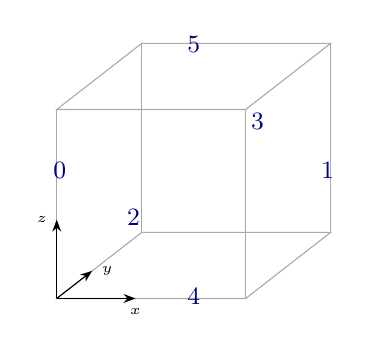
\begin{tikzpicture}[scale=1.0,x={(1cm,0)},y={(0.45cm,0.35cm)},z={(0,1cm)}]
  \draw[DarkGray] (0,0,0) -- (2.4,0,0) -- (2.4,2.4,0) -- (0,2.4,0) -- cycle;
  \draw[DarkGray] (0,0,2.4) -- (2.4,0,2.4) -- (2.4,2.4,2.4) -- (0,2.4,2.4) -- cycle;
  \draw[DarkGray] (0,0,0) -- (0,0,2.4); \draw[DarkGray] (2.4,0,0) -- (2.4,0,2.4); \draw[DarkGray] (2.4,2.4,0) -- (2.4,2.4,2.4); \draw[DarkGray] (0,2.4,0) -- (0,2.4,2.4);
  \node[font=\small,text=NavyBlue] at (-0.5,1.2,1.2) {0};
  \node[font=\small,text=NavyBlue] at (2.9,1.2,1.2) {1};
  \node[font=\small,text=NavyBlue] at (1.2,-0.5,1.2) {2};
  \node[font=\small,text=NavyBlue] at (1.2,3.0,1.2) {3};
  \node[font=\small,text=NavyBlue] at (1.2,1.2,-0.4) {4};
  \node[font=\small,text=NavyBlue] at (1.2,1.2,2.8) {5};
  \draw[-{Stealth[length=1.5mm]}] (0,0,0) -- (1,0,0) node[font=\tiny,below] {$x$};
  \draw[-{Stealth[length=1.5mm]}] (0,0,0) -- (0,1,0) node[font=\tiny,right] {$y$};
  \draw[-{Stealth[length=1.5mm]}] (0,0,0) -- (0,0,1) node[font=\tiny,left] {$z$};
\end{tikzpicture}

\scriptsize Sides 0--5 of a 3D box. A block with only \code{\_0} to \code{\_3} functions leaves sides 4 and 5 undefined, and the run stops at start-up with a message naming the missing key.
\end{column}
\end{columns}
\end{frame}

% 8
\begin{frame}[fragile]{No slip in 3D, and a background flow}
\label{fr:noslip}
\begin{columns}[T,onlytextwidth]
\begin{column}{0.5\textwidth}
\small ``\al{No slip in 3D.} See the \code{input3d} file. Note that \code{VelocityBcCoefs\_0} would set the $x$-component of velocity, and \code{VelocityBcCoefs\_2} would set the $z$-component of velocity.'' (2016) The slide showed \code{VelocityBcCoefs\_1} with all six \code{acoef} $= 1$, \code{bcoef} $= 0$, \code{gcoef} $= 0$: the $y$-velocity is zero on every side.
\vspace{1mm}

\small ``\al{Background flow in the $x$-direction.} In this case we set all of the $a$'s to one. The $x$-component of the velocity should be set to the desired background flow (0.1 in this case). The $y$- and $z$-components should be set to zero.'' (2016)
\begin{lstlisting}[style=inputtiny]
VelocityBcCoefs_0 {                       // boundary conditions for the x-component of the velocity
   acoef_function_0 = "1.0"  ...  acoef_function_5 = "1.0"
   bcoef_function_0 = "0.0"  ...  bcoef_function_5 = "0.0"
   gcoef_function_0 = "0.1"  ...  gcoef_function_5 = "0.1"
}
\end{lstlisting}
\end{column}
\begin{column}{0.48\textwidth}
\small ``\al{Initial conditions.} Previously these have all been set to zero. With the nonzero boundary conditions, we need to change these to the background flow rate.'' (2016)
\begin{lstlisting}[style=inputtiny]
VelocityInitialConditions {
   function_0 = "0.1"   // the x-component
   function_1 = "0.0"   // the y-component
   function_2 = "0.0"   // the z-component
}
\end{lstlisting}
\footnotesize A third \code{function} line, and the same value as the boundaries' $g$. An initial field of $0$ against boundaries at $0.1$ is the impulsive start of chapter 7, in 3D; the 2016 example did it the other way round, a uniform $0.1$ everywhere, which starts the fluid moving through the leaf at $t = 0$.
\vspace{1mm}

\footnotesize Periodic in a direction: the \code{VelocityBcCoefs} entries for its two sides are ignored (next slide), but they must still be present for the file to parse.
\end{column}
\end{columns}
\end{frame}

% 9
\begin{frame}{``Improvements'': the ramp the course promised}
\label{fr:ramp}
\small ``One negative effect of starting with a nonzero background flow is that this has the effect of making a leaf suddenly appear in flow. The result is that very large forces will be generated initially. A possible solution to this (coming soon) would be to start at $u = 0$ and ramp up the velocity smoothly to some nonzero value.'' (2016)
\vspace{2mm}

\footnotesize Delivered, in every example of this series that has a stream: the boundaries carry \code{U\_FLOW*tanh(2*t)} (IB/03, chapter 7), the lid of IB/08 moves as \code{V*tanh(2*t)}, IBFE/10's six sides carry \code{U*tanh(2*t)}, and the initial velocity is zero. The ramp reaches 96\% of its final value at $t = 1$ s; a faster one (\code{tanh(10*t)}) is fine for a stiff structure, a slower one for a floppy sheet.
\vspace{1mm}

\footnotesize In 3D the impulsive start is worse than in 2D for a plain reason: the first step's pressure impulse acts on the whole sheet at once, and a sheet of $N^2$ points has $N$ times the force of a filament of $N$ points on the same tethers. Chapter 11's force files show the spike; chapter 16 shows the abort it can cause.
\end{frame}

% 10
\begin{frame}[fragile]{Domain size and periodic boundaries in 3D}
\label{fr:domain}
\begin{columns}[T,onlytextwidth]
\begin{column}{0.5\textwidth}
\small ``Look at \code{input3d}. \code{x\_lo} sets xmin, ymin and zmin; \code{x\_up} sets xmax, ymax and zmax. \code{Periodic\_dimension} turns on periodic boundary conditions and overrides everything. Set this to zero to turn off periodic BC's.'' (2016)
\begin{lstlisting}[style=inputtiny]
CartesianGeometry {
   domain_boxes = [ (0,0,0) , (N - 1, N - 1, N - 1) ]
   x_lo = -0.5*L, -0.5*L, -0.5*L      // lower end of computational domain
   x_up =  0.5*L,  0.5*L,  0.5*L      // upper end of computational domain
   periodic_dimension = 1, 1, 1
}
\end{lstlisting}
\footnotesize The 2016 file as shown: a cube of $N^3$ coarse cells, periodic in all three directions.
\end{column}
\begin{column}{0.48\textwidth}
\scriptsize What the 2016 input did not say:
\begin{itemize}
  \item with \code{periodic\_dimension = 1, 1, 1} the \code{VelocityBcCoefs} blocks of the previous slides, inflow included, are \al{ignored}: a periodic box has no sides to apply them to. The 2016 leaf therefore saw a uniform initial velocity in a periodic box, not an inflow; chapter 7's rule (``periodic overrides everything'') is the same in 3D. For a stream, set the stream's direction to 0 (IBFE/10: \code{0, 0, 0}; IB/08: \code{1, 1, 0}, periodic across, walls above and below);
  \item the box need not be a cube: IB/08 is $1/8\times1/8\times1$ with \code{domain\_boxes = [(0,0,0), (N/8-1, N/8-1, N-1)]}; the coarse cells are cubes, so the counts follow the lengths;
  \item three numbers everywhere: \code{x\_lo}, \code{x\_up}, \code{periodic\_dimension}, \code{domain\_boxes}, the \code{ratio\_to\_coarser} and patch-size lines of the gridding block, and the \code{largest\_patch\_size} that limits memory per process.
\end{itemize}
\end{column}
\end{columns}
\end{frame}

% 11
\begin{frame}[fragile]{Constructing a sheet: springs and beams in two directions}
\label{fr:sheet}
\begin{lstlisting}[style=pythontiny]
# a rectangular sheet of nx by ny points in the plane x = x0 (the 2016 leaf, rebuilt)
# point (i, j) has number i + nx*j; y = y0 + i*ds, z = z0 + j*ds
with open(f"{name}.vertex", "w", newline="\n") as f:
    f.write("%d\n" % (nx * ny))
    for j in range(ny):
        for i in range(nx):
            f.write("%1.16e %1.16e %1.16e\n" % (x0, y0 + i * ds, z0 + j * ds))
# springs along rows and along columns: (nx-1)*ny + nx*(ny-1) of them
# beams along rows and along columns: (nx-2)*ny + nx*(ny-2) of them
for j in range(ny):
    for i in range(nx - 1):  spring(i + nx*j, i + 1 + nx*j)
    for i in range(nx - 2):  beam(i + nx*j, i + 1 + nx*j, i + 2 + nx*j)
for i in range(nx):
    for j in range(ny - 1):  spring(i + nx*j, i + nx*(j + 1))
    for j in range(ny - 2):  beam(i + nx*j, i + nx*(j + 1), i + nx*(j + 2))
# target points along the centreline j = ny//2
for i in range(nx):  target(i + nx*(ny // 2))
\end{lstlisting}
\footnotesize The same three file types as in 2D (chapter 6), with three coordinates per vertex line and the same spring, beam and target lines; the stiffnesses in the files are the 2D ones per unit width, i.e.\ $K\,\Delta s/\Delta s$ for springs and $k_b\,\Delta s/\Delta s^3$ for beams with the sheet's own spacing. IB/08's generator builds a cylinder the same way (rings of points, \code{x y z} per line, every point a target). What a sheet needs that a filament did not is on the next slide.
\end{frame}

% 11b
\begin{frame}{A sheet is not a filament: shear, twist, and the count of points}
\label{fr:sheet2}
\small Three things a sheet needs that a filament did not:
\begin{itemize}
  \item \al{shear}: springs along rows and columns alone let the rectangle shear into a parallelogram; add diagonal springs (from $(i,j)$ to $(i+1,j+1)$ and $(i+1,j)$ to $(i,j+1)$) if the sheet should keep its angles;
  \item \al{bending in two directions}: beams along rows resist one curvature, beams along columns the other; a sheet that must also resist twist needs the diagonals' beams too;
  \item \al{the point spacing}: $\Delta s \approx \Delta x/2$ of the finest level in \emph{both} directions, so $N_{\mathrm{points}} \sim (L/\Delta s)^2$: a $0.1$ m square leaf at $\Delta x = 1/512$ m is $103\times103 = 10{,}609$ points, and the structure files are a hundred times longer than the leaf's.
\end{itemize}
\vspace{1mm}
\begin{punchbox}
\footnotesize The stiffness bookkeeping of chapter 6 applies per link: a spring along a row of a sheet with spacing $\Delta s$ carries $K/\Delta s$ in the file like any other, and the sheet's stiffness per unit width comes out of how many rows there are. The 2016 generator used the leaf's 2D values unchanged, which is right for a sheet of the same spacing.
\end{punchbox}
\end{frame}

% 12
\begin{frame}[fragile]{Moving target points in 3D}
\label{fr:targets}
\begin{columns}[T,onlytextwidth]
\begin{column}{0.5\textwidth}
\footnotesize ``\al{Update target points.} Another option would be to set the initial and boundary conditions to zero and translate the wing. This could be done with \code{update\_target\_point\_positions}. Just change \code{V} from zero to some value.'' (2016)
\begin{lstlisting}[style=cpptiny]
if (leaf_lag_idxs.first <= lag_idx && lag_idx < leaf_lag_idxs.second)
{
    X_target[0] += V*dt;
}
\end{lstlisting}
\scriptsize Chapter 9a's first form (move the target by $V\Delta t$ each step), with \code{X\_target} now a 3-vector: \code{[0]}, \code{[1]}, \code{[2]} for $x$, $y$, $z$. IB/08 ships exactly this (\code{update\_target\_point\_positions.cpp}, called only when \code{TARGET\_VELOCITY} is not 0): the bristle can be dragged through the fluid instead of the lid dragging the fluid past it.
\end{column}
\begin{column}{0.48\textwidth}
\footnotesize From the 2012 lab ReadMe: ``\al{Simple clap and fling.} \code{Moving\_plates} is a simple proto clap-and-fling IBAMR model. All it does is translate the left wing to the left and the right wing to the right. You all will need to add in the more complex kinematics. When you do so, you may also need to play around with the timestep sizes. You know you have a timestep that is too big when you get an error quickly or when the results don't make sense (very noisy). Timesteps are set by the parameter \code{dt} in the input files (\code{input2d} or \code{input3d}).''
\vspace{1mm}

\footnotesize ``The kinematics of the wings are specified in a C++ function defined in the file \code{update\_target\_point\_positions.C}. If you modify either \code{main.C} or \code{update\_target\_point\_positions.[Ch]}, you will need to recompile the program.''
\vspace{1mm}

\scriptsize IB/07 is the 2D version of that model, with its own README; the 3D one is the same code with three components and the 3D wing files of the next slide.
\end{column}
\end{columns}
\end{frame}

% 13
\begin{frame}[fragile]{The 2012 \code{moving\_plates3d}: files, generator, running}
\label{fr:plates3d}
\vspace{-2mm}
\begin{columns}[T,onlytextwidth]
\begin{column}{0.5\textwidth}
\footnotesize ``\al{Parameters.} The model parameters are defined in a couple of different files. Fluid parameters are defined in the input files (\code{input2d} for the 2D model, \code{input3d} for the 3D model). The material parameters are stored in the files:
\begin{lstlisting}[style=data]
plate3d_left_512.vertex     <=== initial positions of the vertices
plate3d_left_512.spring     <=== list of springs in the model
plate3d_left_512.beam       <=== list of beams in the model
plate3d_left_512.target     <=== list of target points in the model
\end{lstlisting}
These files are generated by a simple Matlab script, where various material parameters are defined. 2D and 3D versions of the Matlab script are in the \code{moving\_plates} folder (\code{generate\_mesh3d.m} and \code{generate\_mesh2d.m}). Run the matlab function twice (setting the if statement to 0 and 1) to make the left wing and the right wing.'' (2012)
\end{column}
\begin{column}{0.48\textwidth}
\footnotesize ``\al{3D code.} For the three-dimensional case, go to \code{.../examples/moving\_plates3d}. Next you can do \code{make clean}, \code{make cleandist}, \code{make main3d}, \code{./main3d input3d}.'' And on the cluster of the day: ``To run a 3D simulation, type \code{make main3d} and \code{bsub -q week -n 16 mpirun ./main3d input3d}. \code{-n 16} will run on 16 processors. I recommend running 16--32 (should be powers of 2).'' (2012)
\vspace{1mm}

\scriptsize Today: \code{cmake} with \code{IBAMR::IBAMR3d} builds \code{main3d} (IB/08's \code{CMakeLists.txt}), and chapter 1's \code{job.slurm} replaces \code{bsub}. The wing of 2012 was a $4{,}661$-point sheet (\code{plate3d\_left\_512.vertex}); the lab's 2014 scripts generalized it to Ellington's beta-function planform (\code{square\_wing.m}, \code{beta\_wing\_mesh.m}: chord, span, the shape parameters $\hat r_1$, $\hat r_2$, an angle of attack), which chapter 20's wings use. ``Run the function twice'' is chapter 9a's two-structure pattern: one file set per wing, both named in \code{structure\_names}.
\end{column}
\end{columns}
\end{frame}

% 14
\begin{frame}{IB/08, the 3D IB example of this series: a bristle in a sheared box}
\label{fr:ib08}
\begin{columns}[T,onlytextwidth]
\begin{column}{0.56\textwidth}
\footnotesize From its README: ``One glycocalyx fiber, a cylinder made of 13,600 target points, stands on the floor of a box of fluid. The lid of the box slides sideways, so the fluid is sheared past the fiber. The box is periodic in $x$ and $y$, so the run models one fiber in an endless square array of fibers. It shows a box that is not a cube, periodic and wall boundaries together, a moving wall, target points in 3D, and 3D output for VisIt.''
\begin{itemize}\footnotesize
  \item Box $1/8\times1/8\times1$ m, periodic in $x$ and $y$; the floor fixed, the lid moving at $V\tanh(2t)$, $V = 0.1$ m/s.
  \item Grid: 3 levels, ratio 4, $4\times4\times32$ coarse cells, $\Delta x = 1/512$ m on the finest level, which covers only $40\times40\times96$ cells around the fiber; $161{,}280$ cells in all.
  \item Fluid $\rho = 1000$, $\mu = 40$; $\mathrm{Re} = 0.061$ on the fiber's height.
  \item Fiber: radius $0.0132$ m, height $0.156$ m, 160 rings of 85 points, every point a target with $\kappa = 3.19\times10^4$.
  \item 20,000 steps of $10^{-5}$ s, about 20 minutes on 4 cores.
\end{itemize}
\end{column}
\begin{column}{0.42\textwidth}
\scriptsize What its README teaches that a 2D run could not:
\begin{itemize}
  \item \al{how long the flow takes to arrive}: the lid's motion diffuses down with $\nu = 0.04$; the 1D solution gives $0.5\%$ of the final shear at the fiber's top at $1$ s, $55\%$ at $4$ s, $96\%$ at $10$ s. The course ran 10 s, a million steps; the default here stops at $0.2$ s, before the flow reaches the fiber, and \code{SHEAR\_START = 1} starts from the steady shear instead;
  \item \al{a 3D stiffness trap}: the target stiffness in the file is $\kappa/ds$ with the generator's $ds = $ radius$/84$, not the points' true spacing around the ring ($6.2$ times larger); kept so that the files match every earlier version, and flagged;
  \item \al{3D output}: \code{viz\_IB3d}, \code{hier\_data\_IB3d} with three numbers per point, the fiber as a mesh in VisIt (chapter 27).
\end{itemize}
\end{column}
\end{columns}
\end{frame}

% 15
\begin{frame}[fragile]{IB/08's \code{input3d}: what differs from 2D, line by line}
\label{fr:input3d}
\begin{lstlisting}[style=inputtiny]
N = 32                              // coarse cells in z; x and y have N/8
...
CartesianGeometry {
   domain_boxes = [ (0,0,0) , (N/8 - 1, N/8 - 1, N - 1) ]
   x_lo = -L/16, -L/16, -L/2        // lower end of computational domain
   x_up =  L/16,  L/16,  L/2        // upper end of computational domain
   periodic_dimension = 1, 1, 0     // periodic across, walls above and below
}
GriddingAlgorithm {
   ratio_to_coarser { level_1 = REF_RATIO, REF_RATIO, REF_RATIO ... }
   largest_patch_size { level_0 = 512, 512, 512 }
   smallest_patch_size { level_0 = 8, 8, 8 }
   ...
}
VelocityBcCoefs_0 { ... six acoef, six bcoef, six gcoef; gcoef_function_5 = "V*tanh(2*t)" }
VelocityBcCoefs_1 { ... }
VelocityBcCoefs_2 { ... }           // the block 2D does not have
VelocityInitialConditions { function_0 = "0.0"  function_1 = "0.0"  function_2 = "0.0" }
\end{lstlisting}
\footnotesize Read it on the next slide.
\end{frame}

% 15b
\begin{frame}{IB/08's \code{input3d}, read}
\label{fr:input3d2}
\small
\begin{itemize}
  \item \code{domain\_boxes} with three indices; the counts in $x$ and $y$ are an eighth of the count in $z$ because the box is;
  \item \code{x\_lo}, \code{x\_up}, \code{periodic\_dimension} with three entries;
  \item every \code{ratio\_to\_coarser}, \code{largest\_patch\_size}, \code{smallest\_patch\_size} line with three entries;
  \item a third \code{VelocityBcCoefs} block, each block with six sides; the lid's motion is \code{gcoef\_function\_5} of the $x$-component (side 5 is $z$ upper);
  \item a third \code{function} in the initial conditions;
  \item the program is built as \code{main3d} (\code{IBAMR::IBAMR3d}); \code{NDIM} is 3 in every loop of \code{main.cpp} and the update function, with no edits.
\end{itemize}
\vspace{1mm}
\footnotesize The muParser functions may use \code{X\_0}, \code{X\_1}, \code{X\_2} and \code{t}; a lid velocity that varies across the lid (\code{V*tanh(2*t)*(1 - 4*X\_1*X\_1/(L*L))}) is one line.
\end{frame}

% 16
\begin{frame}{IBFE/10, the 3D IBFE example: a plate in a flow tank}
\label{fr:ibfe10}
\small From its README: ``A thin elastic plate stands across a uniform stream in a 3D flow tank. A band across the middle of the plate is held in place by a tether (target) force, and the parts above and below the band are free to bend with the flow. It reads a tetrahedral mesh made with gmsh, uses a compressible neo-Hookean material, applies a tether force to part of the body, and writes the plate's motion to an ExodusII file.''
\begin{itemize}\footnotesize
  \item Tank $32\times16\times16$, not periodic; six sides at $(U\tanh(2t), 0, 0)$ with $U = 0.1$; $\rho = 1$, $\mu = 0.01$, $\mathrm{Re} = 20$ on the plate's width.
  \item Grid: 3 levels, ratio 4, $32\times16\times16$ coarse cells, $\Delta x = 1/16$ on the finest level around the plate.
  \item Plate $0.125$ thick, $2\times2$, 3,386 nodes and 11,481 tetrahedra; 5,000 steps, 30--50 minutes on 4 cores.
\end{itemize}
\vspace{1mm}
\footnotesize It is the 3D version of the 2016 leaf with a different structure model: the sheet of springs and beams becomes a solid with a stress law (chapter 19), the line of target points a tethered band (chapter 22), and the \code{.vertex} file a gmsh mesh (chapter 18). The input file's fluid half is the one on the previous slide with \code{periodic\_dimension = 0, 0, 0} and a stream on all six sides.
\end{frame}

% 17
\begin{frame}{What 3D costs}
\label{fr:cost}
\footnotesize
\begin{itemize}
  \item \al{Cells}: a uniform grid of $N$ cells per side has $N^3$: $512^3 = 1.3\times10^8$, against $512^2 = 2.6\times10^5$ in 2D, five hundred times more. Adaptive refinement is what makes 3D possible: IB/08's finest level covers $40\times40\times96 = 1.5\times10^5$ cells of a $64\times64\times512$ box, and the whole hierarchy $1.6\times10^5$.
  \item \al{Points}: a sheet has $(L/\Delta s)^2$ points, a surface $(L/\Delta s)^2$, a volume $(L/\Delta s)^3$ (IBFE); IB/08's bristle, a surface, has $13{,}600$.
  \item \al{Steps}: the time step limit is the same as in 2D (chapter 5), set by $\Delta x$ and the stiffness, so a run of the same physical time has the same number of steps; each step costs the number of cells and points. IB/08: $0.05$ s per step on 4 cores for $1.6\times10^5$ cells; the course's 10 s were a million steps, a day on 16 cores.
  \item \al{Memory}: every cell carries velocity, pressure, the tagging and the forcing; a million cells is a few hundred MB per field set. \code{largest\_patch\_size} bounds what one process holds; a 3D run is what the 2012 advice ``16--32 processors, powers of 2'' and Puma's nodes (chapter 1) are for.
  \item \al{Output}: a \code{viz\_IB3d} frame of $10^6$ cells is tens of MB; 50 frames of IB/08 are manageable, 500 are not. Write \code{hier\_data} often and the fields rarely (chapter 11).
\end{itemize}
\begin{punchbox}
\footnotesize The first 3D run should be short (IB/08's $0.2$ s), on the coarsest grid that resolves the structure, with one frame written: check the geometry, the sides, the ramp and the step before spending a day of cluster time. Then chapter 16's convergence test.
\end{punchbox}
\end{frame}

% 18
\begin{frame}{3D output and where it goes next}
\label{fr:output}
\small
\begin{itemize}
  \item \code{hier\_data\_IB3d/X.NNNNN} and \code{F.NNNNN}: three numbers per point, read with \code{ndim = 3} by chapter 11's readers; the lab's 2014 3D script summed \code{A(1:3:end)}, \code{A(2:3:end)}, \code{A(3:3:end)}.
  \item \code{viz\_IB3d/dumps.visit}: the fields on the 3D hierarchy; \code{lag\_data.visit}: the structures as 3D point meshes (IB/08's \code{glyco\_512\_vertices}; a \code{\_mesh} of edges exists only for structures with springs, chapter 28).
  \item \code{IB3d.log} and the \code{integral\{F\}} lines with three components.
  \item The IBFE examples write the solid to an ExodusII file (\code{.ex2}) with libMesh (chapter 28).
\end{itemize}
\vspace{1mm}
\footnotesize Chapter 27 is the VisIt chapter for 3D: a slice through the box (the 2015 note \emph{Taking a 2D slice from 3D IBAMR with VisIt}), isosurfaces of vorticity magnitude, a mesh plot of the structure with the slice behind it, and the camera. The 2012 ReadMe's advice still holds: ``open up the \code{lag\_data.visit} database, make a `mesh' plot: you should be able to make a line plot of the springs and a point plot of the vertices; \code{dumps.visit} plots the adaptive mesh, velocities, vorticities, etc.''
\end{frame}

% 19
\begin{frame}{What can go wrong}
\label{fr:wrong}
\scriptsize
\begin{tabular}{@{}L{0.32\textwidth}L{0.6\textwidth}@{}}
\toprule
The mistake & What happens\\
\midrule
\code{periodic\_dimension = 1, 1, 1} with an inflow & the inflow is ignored; the fluid moves only if the initial condition says so (the 2016 input). Set the stream's direction to 0\\
a \code{VelocityBcCoefs} block with four sides & the run stops at start-up asking for \code{acoef\_function\_4}; copy all six\\
no \code{VelocityBcCoefs\_2} & the same, for the $z$-component\\
two numbers in \code{x\_lo} or \code{domain\_boxes} & a parse error, or a box with the wrong shape\\
initial velocity $\neq$ boundary velocity & chapter 7's impulsive start; use the ramp on the boundary and zero inside\\
$\Delta s$ from the wrong length (IB/08's radius$/84$) & a stiffness several times off; compute the spacing from neighbouring points\\
a sheet without diagonals or cross beams & it shears or twists freely; add them if the physics needs them\\
a 2D time step in 3D & the same $\Delta x$ allows the same $\Delta t$; but a finer $\Delta x$ chosen to fit memory does not\\
the course's 10 s on a laptop & a million steps; run $0.2$ s first, then the cluster\\
one process for a million cells & memory; use 16--32 processes and \code{largest\_patch\_size}\\
\bottomrule
\end{tabular}
\end{frame}

% 20
\begin{frame}{Homework}
\label{fr:hw}
\begin{columns}[T,onlytextwidth]
\begin{column}{0.56\textwidth}
\footnotesize From the 2012--2016 courses and this chapter (Appendix C collects the full set):
\begin{enumerate}
  \item IB/08: run the default $0.2$ s, then \code{SHEAR\_START = 1}, and compare the force on the fiber (chapter 11, \code{ndim = 3}) at the end of each.
  \item IB/08: drag the fiber instead of the lid (\code{TARGET\_VELOCITY}), with the lid at rest; is the force the same?
  \item Build the 2016 sheet with slide \ref{fr:sheet}'s recipe ($0.1$ m square, $\Delta s = \Delta x/2$ at $\Delta x = 1/256$ m), tether its centreline, put it in IB/08's box with a stream in $x$ (\code{periodic\_dimension = 0, 1, 0}), and run $0.5$ s. Report the number of points, cells and the time per step.
  \item Add diagonal springs to the sheet and compare the shape at $0.5$ s.
  \item IBFE/10: halve the plate's shear modulus and compare the bending (chapter 22).
\end{enumerate}
\end{column}
\begin{column}{0.43\textwidth}
\begin{punchbox}
\scriptsize What to hand in: the \code{input3d} blocks you changed, the generator loop, the point and cell counts, the time per step on the cores you used, and one VisIt image with a slice and the structure.
\end{punchbox}
\scriptsize Extension: the two wings of the 2012 model, translated apart in 3D (IB/07's update function with \code{X\_target[0]}), on a coarse grid.
\end{column}
\end{columns}
\end{frame}

% 21
\begin{frame}{Rules of thumb}
\label{fr:thumb}
\small
\begin{itemize}
  \item Three numbers wherever 2D had two; six sides, $2d$ lower and $2d + 1$ upper; a third component block.
  \item Periodic overrides the sides: a stream needs its direction non-periodic.
  \item Ramp the boundary, start the fluid at rest.
  \item A sheet is rows and columns of springs and beams, plus diagonals if it must not shear.
  \item $\Delta s \approx \Delta x/2$ in every direction of the structure; points grow as $(L/\Delta s)^2$.
  \item Refine only around the structure; check the cell count in the log before the long run.
  \item Short first, coarse first, one frame first; then the cluster, 16--32 processes.
  \item Positions and forces have three numbers per point; VisIt needs a slice.
\end{itemize}
\end{frame}

% 22
\begin{frame}{Summary}
\label{fr:summary}
\footnotesize
\begin{enumerate}
  \item A 3D IBAMR run is the 2D one with a third coordinate everywhere: in the domain and gridding blocks, in six-sided boundary-condition blocks for three components, in a third initial condition, and in structure files with $x\,y\,z$ per point. The method does not change.
  \item The course's 3D leaf (a sheet of springs and beams tethered along its midline) and the lab's clap-and-fling plates (two wings translated apart) are the 2D examples of chapters 7 and 9a in 3D; the recipes for the sheet, the target motion and the two-structure input are given here, and IB/08 and IBFE/10 are the runs.
  \item Periodic directions ignore the sides; a stream needs a non-periodic direction, a ramp and a fluid at rest.
  \item The cost is the point: $N^3$ cells and $(L/\Delta s)^2$ points, the same number of steps as in 2D, so adaptive refinement, a short coarse first run and a cluster are part of the method.
  \item The output has three numbers per point and needs a slice to be seen; chapters 11 and 27 do that.
\end{enumerate}
\begin{homebox}
\footnotesize Next, chapter 13: adding mass, where points get a mass of their own and fall under gravity.
\end{homebox}
\end{frame}

% 23
\begin{frame}{What changed since the older course notes}
\label{fr:changed}
\footnotesize
\begin{itemize}
  \item The 2016 lecture's input fragments are quoted and completed: the side rule ($2d$, $2d+1$), the third component block, the three-entry lines of the gridding block, and the fact that its \code{periodic\_dimension = 1, 1, 1} silently ignored the inflow it set.
  \item ``Improvements (coming soon)'' is delivered: every example with a stream ramps it.
  \item The sheet generator, whose file is gone, is rebuilt as a recipe with the shear and twist caveats; the 2012 moving-plates model is described from the lab ReadMe with its wing files and the lab's 2014 planform scripts named.
  \item IB/08 and IBFE/10 replace the unavailable examples, with measured run times and the shear-flow timing that explains the course's 10-second runs.
  \item New: the cost slide, the output slide, the what-can-go-wrong table, and the homework that builds the 2016 sheet.
  \item Left out: the 2013 3D deck (unreadable format), the 2012 ssh walk-through (chapter 1), and the lab machine names and credentials of the 2012 decks.
\end{itemize}
\end{frame}

% 24
\begin{frame}{Recordings (listed, not incorporated)}
\label{fr:videos}
\small The front matter's video list (chapter 0.1) has no recording of the 2016 3D lecture. The 3D material that was recorded is VisIt's, and belongs to chapter 27: \code{2-Video\_Visualizing3Ddata.mp4} (2018-02-26, 258 MB) and its 2019 copy \code{Lecture 2-Video\_Visualizing3Ddata.mp4} (2019-07-03), and the 2022 VisIt tutorial's \code{3D flow.mp4} (2023-07-25, 40 MB). The decks they go with (\emph{VISIT in 3D with IBAMR}, 2018 and 2020; \emph{Taking a 2D slice from 3D IBAMR with VisIt}, 2015) are chapter 27's sources.
\end{frame}

% 25
\begin{frame}{References}
\label{fr:refs}
\scriptsize
\begin{itemize}
  \item This series: \code{examples/IB/08-glycocalyx-3d} and \code{examples/IBFE/10-flow-tank-plate-3d} (READMEs with the measured numbers); chapters 7, 9a, 11, 15, 18, 22, 27, 28.
  \item IBAMR: \code{examples/IB/explicit/ex7} (3D posts held by target points), \code{examples/IBFE/explicit/ex4}, \code{ex5} (3D elastic bodies in a stream); the input keys of \code{CartesianGeometry}, \code{GriddingAlgorithm} and \code{muParserRobinBcCoefs}, \url{https://ibamr.github.io/docs}.
  \item C. P. Ellington, \emph{The aerodynamics of hovering insect flight. II. Morphological parameters}, Phil.\ Trans.\ R.\ Soc.\ B 305 (1984) 17--40 (the beta-function planform of the lab's wing scripts).
  \item Sources: \emph{IBAMR boundary conditions / 3D simulations} (public folder 8, 2016, 12 slides); the lab's \emph{IBAMR ReadMe} deck (2012; the moving-plates model, kinematics, parameters, 3D code, cluster runs); \emph{Math769 3D} (2013; unreadable); the lab's 3D wing files and scripts (2012--2014).
\end{itemize}
\end{frame}

\end{document}
